\section{Meio ambiente e educação ambiental}

Segundo \citeaa{McReynolds1999}, A Sociologia do meio ambiente é uma área antiga, apesar de nova. Marx e Engels (\citeaa{Marx1961}), Weber e Durkheim (1954,1982), todos escreveram sobre o relacionamento entre sociedades humanas e o meio ambiente natural. Contudo, o termo "Sociologia do meio ambiente" não foi utilizado até 1971. Em 1976, A Sociedade Americana de Sociologia designou uma seção para a área. Em 1978, Catton e Dunlop publicaram a primeira tentativa de proporcionar uma definição explícita da área de sociologia do meio ambiente. E, não foi antes de 1990 que a Sociedade Internacional de Sociologia formou o seu primeiro grupo com interesse específico em sociologia do meio ambiente.\\

Hoje em dia, a sociologia do meio ambiente procura incorporar mais variáveis científicas naturais, perspectivas e até paradigmas em seus métodos, teorias e literatura. O aumento do crescimento e do interesse em perspectivas multi e interdisciplinares também acrescentou em amplitude para o aprofundamento da sociologia do meio ambiente. Esta expansão fez da sociologia ambiental um emaranhado de disciplinas com bases crescentes na biologia, ecologia, ciência política, antropologia, psicologia, feminismo e outras. Apesar da aparência pós-moderna, a sociologia do meio ambiente ainda pretende ser a única linha de pensamento viável capaz de proporcionar uma perspectiva macro ou além, conforme \citeaa{CATTON1978} e \citeaa{REDCLIFT1997}. \\

A Sociologia do meio ambiente tem sido definida de diversas maneiras. Entre as várias definições, \citeaa{BUTTEL1996}  proporciona um começo útil. Ele nota que hoje em dia a essência da sociologia do meio ambiente tem sido de recuperar e revelar a materialidade da estrutura e vida social, e o faz de maneira a produzir entendimentos relevantes de modo a resolver problemas ambientais. Esta definição reconhece ao mesmo tempo a centralização da verdadeira natureza física do meio ambiente e o papel representado pelas construções sociais da natureza.\\

A união da natureza física e das construções sociais da natureza permanece atualmente como a principal preocupação para a sociologia ambiental. Na verdade, a habilidade de unir estes conceitos aparece como o centro da pretensão da área de ser a melhor das áreas da sociologia a se aplicar a um dos maiores problemas mundiais - o declínio do meio ambiente. Com o final da Guerra Fria, as preocupações sobre o aquecimento global e mudanças no meio ambiente mundial tomaram o lugar das preocupações com a guerra nuclear. Sendo assim, a sociologia do meio ambiente tem ocupado o cenário central na relação dos problemas mundiais [\citeaa{VAILLANCOURT1995}].\\

Neste contexto, a sociologia do meio ambiente está preocupada com uma vasta gama de questões, campos de estudo e disciplinas. Se por um lado essa amplitude é excitante, é fácil se perder no labirinto do que veio a se tornar a sociologia do meio ambiente. Nas páginas seguintes apresento uma bibliografia de fontes e uma lista de jornais que relevam o conhecimento da área. Nenhum deles pretende ser exaustivo. Ao contrário, eles têm a intenção de proporcionar ao estudante novo e intermediário da área um acesso mais direto à literatura histórica crítica, teórica e metodológica. Com essas bases, espera-se que o leitor fique mais preparado para pesquisar este crescente e importante campo da sociologia.\\

\citeaa{Geraldino2014} aborda o meio ambiente com a seguinte definição:
Sem adentrar o campo da etimologia, tomando a expressão como equivalente de
ambiente e meio, partiremos do pressuposto de que a essência do conceito deve ser inicialmente
investigada sob dois aspectos: um negativo e outro positivo. Isso quer dizer que, ao
questionar o que é o meio ambiente, devemos, antes de tudo, ter estabelecido a que coisa
este se faz meio e, portanto, a que coisa ambienta. Afinal, como bem defendeu Richard
Hartshorne (1978, p. 66), “o conceito de meio não tem sentido, exceto em referência
àquilo que ele envolve”; ou, como quis Amos Rapoport (19781 apud Holzer, 1997, 80), tal
conceito define-se basicamente por ser “qualquer condição ou influência situada fora do
organismo, grupo ou sistema que se estuda”. Então, só podemos começar dizer algo sobre
o meio ambiente após termos afirmado outro ente ao qual este se faz como não sendo.
Meio ambiente, assim, não pode ser compreendido como uma coisa entre coisas; algo que
nos permita optar por começar a investigar seu ser positivamente, tal como podemos fazer
com uma cadeira ou com um cachorro. Pois, por exemplo, na tentativa de dizer o que são ambos, podemos começar nos referindo a eles por juízos positivos como “uma cadeira é
algo feito para sentar” ou “o cachorro é um animal que late”. Todavia, este procedimento
não cabe à definição de meio ambiente. Para afirmar algo devemos antes tê-lo tratado negativamente.
Ou seja, meio ambiente primeiro tem que não ser algo, para depois ser. Esta
é sua elementar condição: a negativa. Embora que já nesta própria se assente, em concomitância,
outra de igual valor: a relativa. Pois, ao dizermos “meio não é algo”, estamos de
forma implícita dizendo que meio é relativo a algo. Daí tudo aquilo que não é aquela(e) cadeira/
cachorro, faz-se como ambiente daquela(e) cadeira/cachorro. Relatividade e negatividade
fazem-se, portanto, como os princípios necessários para toda e qualquer tentativa
de definição deste conceito.\\

Se para encontrarmos as propriedades do meio ambiente devemos antes afirmar as características
do tipo de ser do qual se faz negativo e relativo, então, chegamos à necessidade
de especificar de que tipo de ser falamos. Assim, observando o ambiente que nos cerca, que se
estende dos papéis e canetas próximos à imensidão incógnita do universo, verificaremos uma
pluralidade de seres dos quais vamos aqui distinguir agrupando-os em três tipos fundamentais,
a saber: (i) seres inanimados ou não-vivos, (ii) seres vivos ou orgânicos, (iii) seres conscientes
ou humanos. Esse deslindar tripartido é realizado a partir da aplicação de dois recortes arbitrários
no real: o recorte da vida e o da consciência. Fazendo que tenhamos para analisar três tipos
de meios com suas respectivas relações particulares: (i) o meio em que se encontram os seres
não-vivos, (ii) o meio relativo aos seres vivos, (iii) e o meio ao qual ambienta os seres humanos.\\

Completa \citeaa{Geraldino2014} Há no ser humano uma irredutibilidade ao meio. Ou seja, ao homem, não se pode dizer
plenamente “diz-me onde estás e dir-te-ei quem és”, pois isso é ecologia, e não se aplica ao
animal tombado dessa esfera. Portanto, se de fato quisermos compreender o meio ambiente
no qual se encontra um indivíduo ou um grupo, devemos antes questionar suas projeções de
ser; devemos tentar compreender o ir ao futuro que elegeu(ram) como fim possível/faltante e
retornar ao presente, captando neste os entraves e caminhos que devrá(ão) transpor e seguir
para alcançá-lo(s).\\

Já \citeaa{Dias1994}  diz, no tocante a \textbf{educação ambiental}, que a "Educação Ambiental se caracteriza por
incorporar as dimensões sociais, políticas, econômicas,
culturais, ecológicas e éticas, deixando claro que ao discutir
qualquer problema ambiental é fundamental a consideração
de todos estes aspectos." Segundo este autor, "a maior parte
dos problemas ambientais tem suas raízes na miséria que,
por sua vez, é gerada por políticas e problemas econômicos,
concentradores de riqueza e responsáveis pelo desemprego
e degradação ambiental."\\

Pode-se também definir a educação ambiental, nas palavras de \citeonline{Magalhaes2018}, como um processo
onde o educando obtém conhecimentos acerca das
questões ambientais e assim passa a ter um novo
entendimento acerca do meio ambiente, se tornando um
agente transformador referente à preservação do meio
ambiente e de seus recursos naturais. \\

\citeaa{Gadotti2000} explica que educação ambiental vai muito além do conservacionismo
Trata-se de uma mudança radical de mentalidade em
relação à qualidade de vida, que está diretamente ligada
ao tipo de convivência que mantemos com a natureza e
que implica em atitudes, valores, ações. Trata-se de uma
opção de vida por uma relação saudável e equilibrada,
com o contexto, com os outros, com o ambiente mais
próximo, a começar pelo ambiente de trabalho e
doméstico.\\

\subsection{Demonstrações de educação ambiental}

Não faltam demonstrações de preocupação com o meio ambiente, como o visto em \citeaa{AgenciaBrasilia20200424Horta}, em que a Secretaria de Meio Ambiente do Distrito Federal (Sema) e operadores da Logística Reversa (LR) de eletroeletrônicos se preparam para assinar o Termo de Compromisso para a gestão deste tipo de resíduo no Distrito Federal. Este poderá ser o primeiro celebrado no DF e tem como meta ampliar o recolhimento de eletroeletrônicos em comércios varejistas, órgão públicos e postos de combustíveis em conformidade com o Plano Distrital de Gestão Integrada de Resíduos Sólidos (PDGIRS).\\

Como demonstrado na Figura~\ref{fig:logistica-reversa}, logística reversa é um conjunto de procedimentos e meios para recolher e dar encaminhamento pós-venda ou pós-consumo ao setor empresarial, para reaproveitamento ou destinação correta de resíduos.

\begin{figure}[h]
    \centering
    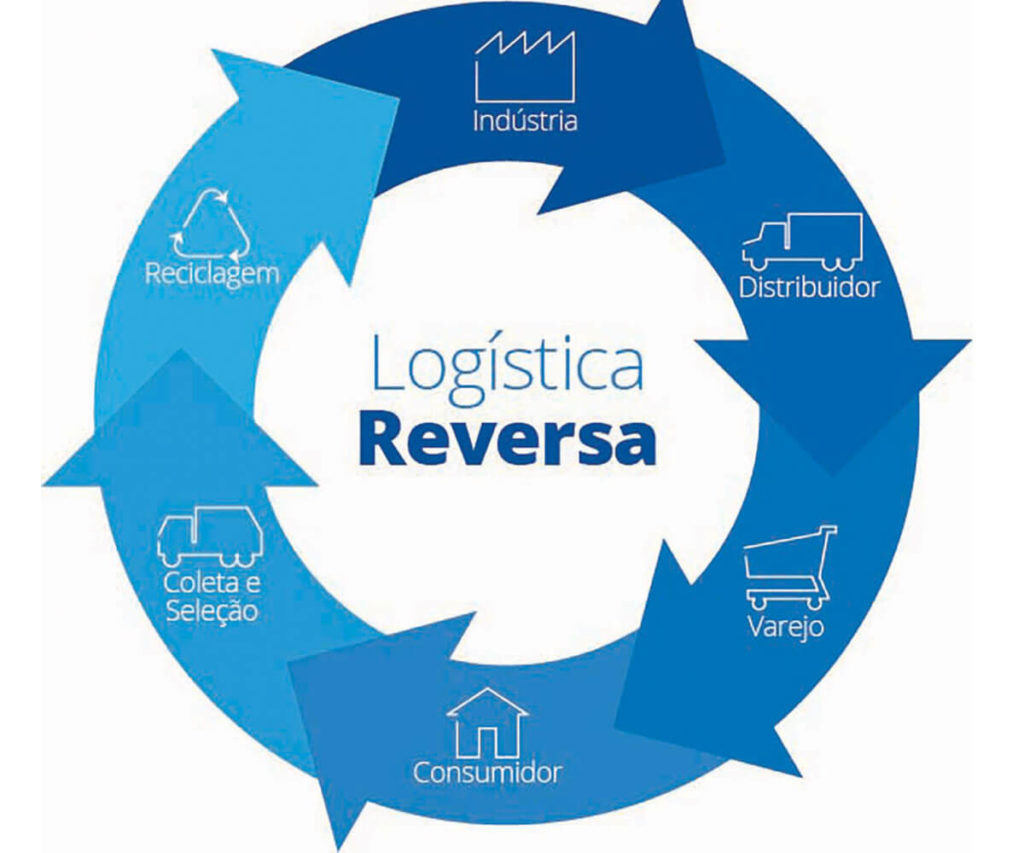
\includegraphics[width=0.7\linewidth]{fig/Logistica-Reversa}
    \caption[Conceito de logística reversa]{Conceito de logística reversa}
    \label{fig:logistica-reversa}
\end{figure}



Nas palavras de \citeaa{Magalhaes2018} "A educação ambiental impacta não apenas no meio em que vivemos, mas está diretamente ligada à
sobrevivência humana, e precisa estar presente no ensino de forma incisiva.
A introdução da educação ambiental nos primeiros anos da educação infantil potencializa o
processo de ensino-aprendizagem, uma vez que o ambiente escolar é um dos meios de integração e
conscientização mais completos para abordar as problemáticas entre a relação homem e natureza.
Quando a educação ambiental é aplicada desde o início do processo de educação e se torna
constante nos anos subsequentes, a aprendizagem transforma-se permanentemente.
É evidente que as mudanças no meio ambiente ocorrem de forma lenta e gradativa, mas quanto
antes iniciado o processo de educação e conscientização da população, maiores são as chances de
sucesso. Assim, é de fato extremamente importante que a Educação Ambiental seja inserida desde
os primeiros anos da educação infantil.
Entretanto, este não é um dever apenas da escola: é fundamental que todos os segmentos da
sociedade em que a criança está inserida se envolvam e busquem este objetivo comum. Está
conscientização das crianças também é um dever dos pais e da sociedade em geral."\\

\citeaa{Gadotti2000} afirma:

\begin{citacao}
    Educação ambiental vai muito além do conservacionismo Trata-se de uma mudança radical de mentalidade em relação à qualidade de vida, que está diretamente ligada ao tipo de convivência que mantemos com a natureza e que implica em atitudes, valores, ações. Trata-se de uma opção de vida por uma relação saudável e equilibrada, com o contexto, com os outros, com o ambiente mais próximo, a começar pelo ambiente de trabalho e doméstico.
\end{citacao}

O acúmulo do grande descuido ambiental faz com que a temática de conservação do meio ambiente esteja em evidência há alguns anos. São constantes as discussões que abordam a preservação ambiental e a sustentabilidade, bem como as explanações cada vez mais claras sobre as consequências negativas da falta de preservação dos recursos naturais. Cresce de forma considerável os questionamentos de como realizar mudanças significativas que auxiliem na preservação e renovação do meio ambiente.\\

São os recursos ambientais que possibilitam boas condições de sobrevivência, portanto, se torna imprescindível a necessidade da conscientização de preservar o que ainda temos e de minimizar os impactos ambientais das ações negativas que acontecem diariamente em todo o mundo.  Atualmente, a maneira mais eficiente para conscientização dos indivíduos é a educação ambiental.\\

Dias (1994), diz que a Educação Ambiental se caracteriza por incorporar as dimensões sociais, políticas, econômicas, culturais, ecológicas e éticas, deixando claro que ao discutir qualquer problema ambiental é fundamental a consideração de todos estes aspectos. Segundo este autor, “a maior parte dos problemas ambientais tem suas raízes na miséria que, por sua vez, é gerada por políticas e problemas econômicos, concentradores de riqueza e responsáveis pelo desemprego e degradação ambiental”.\\

Diante de todas estas preocupações, buscamos mostrar a necessidade de que a educação ambiental seja trabalhada já nos primeiros anos da educação infantil, fazendo com que as crianças de hoje reflitam sobre as ações do ser humano e seus impactos no meio ambiente, visando formar novos cidadãos conscientes que no futuro serão adultos com ações melhores comparadas aos adultos que temos hoje.\\
